\documentclass[preprint]{aastex}
\usepackage{amsmath}
\usepackage{verbatim}
\usepackage{graphicx}
\newcommand{\lnnu}{\ln{\nu}} 
\usepackage[OT2,T1]{fontenc}
\usepackage{url}

\DeclareSymbolFont{cyrletters}{OT2}{wncyr}{m}{n}
\DeclareMathSymbol{\Sha}{\mathalpha}{cyrletters}{"58}
\begin{document}

\title{Beating Out Redshift Drift}
\section{Spatial Heterodyne Spectroscopy}
\label{SHS:sec}
\subsection{Measuring Redshift}
The precision measurement of redshift from a spectral line is hampered by line broadening. 
Redshift can also be measured through the sum and the difference of observed wavenumbers of two lines whose restframe wavenumbers are known:
\begin{equation}
(1+z)=\frac{\sigma_{10}+\sigma_{20}}{\sigma_{1}+\sigma_{2}}=\frac{\sigma_{10}-\sigma_{20}}{\sigma_{1}-\sigma_{2}},
\label{redshift:eqn}
\end{equation}
where $\sigma_i$ is the observed and $\sigma_{i0}$ the restframe wavenumber of line $i$.
At face value, the measurement of $\sigma_1\pm\sigma_2$ should be expected to suffer larger uncertainty than that of the wavenumber
of a single line.  To counter this expectation, we consider a scenario where: The experimental setup has an output that is naturally sensitive
to $\sigma_1\pm\sigma_2$ while being immune to certain systematic uncertainties found in traditional dispersion spectrographs;
Redshifts are measured from the relative shift of a single line profile common to two lines of a doublet.


\subsection{Signal}
%Specifically,  when using a single feature to measure redshift the shape of the line profile
%contributes uncertainty.
%In contrast,  two lines of a doublet share a common line profile (in log-wavenumber) determined by the kinematics of the
%atoms that produce both emissions:
%the redshift measurement depends not directly on the profile but in its relative shift between the two lines .

We consider Spatial heterodyne spectroscopy (SHS) \citep{1990SPIE.1235..622H}
as a means to get a direct measurement of  $\sigma_1\pm\sigma_2$.
Conceptually, the SHS can be understood as as interferometer with the  mirrors replaced by diffraction gratings.
(Practically we assume an interferometer configuration that  avoids the 50\% light loss inherent to  Michelson interferometers.)
The gratings have line-spacing $d$ and both are tilted
by $\theta$ with respect to the optical axis.  The deflected light from each grating exits the interferometer as a plane wave
propagating with angle $\gamma$ away from the optical axis,  given by the grating equation
\begin{equation}
\sigma\left(\sin{\theta}+\sin{\left(\theta-\gamma\right)}\right)=m/d,
\end{equation}
where $\sigma$ is the wavenumber and $m$ the diffraction order.
The angle of the emergent wave can be re-expressed as
\begin{equation}
\sin{\gamma}=-\cos{\theta} \left(\frac{m}{d\sigma} - \sin{\theta} \right)+ \sin{\theta}\sqrt{1-\left(\frac{m}{d\sigma} -\sin{\theta} \right)^2},
\end{equation}
which is useful in calculations.

The two wavefronts from the two gratings, incident on the detector at angles $-\gamma$ and $\gamma$, constructively interfere to make a fringe
pattern with  frequency
\begin{equation}
f_x=2\sigma\sin{\gamma}.
\end{equation}
For an input spectrum of $B(\sigma)$, the intensity seen at the detector at position $x$ is
\begin{equation}
I(x)=\frac{1}{\Delta x}\int_{0}^{\infty} B(\sigma)\left(1+\cos{\left(2 \pi x (2\sigma \sin{\gamma})\right)}\right)d\sigma,
\end{equation}
where for simplicity we assume a square collimated beam that covers
a range  $\Delta x \gg \left(2\sigma \sin{\gamma}\right)^{-1}$.
The Littrow wavenumber $\sigma_0$ is defined such that $2\sigma_0\sin{\theta}=m/d$, $\gamma=0$ and no fringe patterns are produced.

\subsection{Toy Example}
\label{toy:sec}
Consider a toy example where the input signal consists of two $\delta$-functions with the same intensity
\begin{equation}
B(\sigma)=\delta(\sigma_1)+\delta(\sigma_2).
\end{equation}
The output signal density in this case is
\begin{align}
I(x)&=\frac{1}{\Delta x}\left[2+ \cos{\left(2 \pi (2\sigma_1  \sin{\gamma_1}x \right)}+ \cos{\left(2\pi (2  \sigma_2  \sin{\gamma_2})x \right)}\right]\\
&=\frac{2}{\Delta x}\left[1+ \cos{\left(2 \pi  (\sigma_1  \sin{\gamma_1}+ \sigma_2  \sin{\gamma_2})x \right)}\times\cos{\left(2\pi  (\sigma_1  \sin{\gamma_1}- \sigma_2  \sin{\gamma_2})x\right)}\right].
\end{align}
The two mixing of the sinusoidal outputs of the two lines results in two beat frequencies $(\sigma_1  \sin{\gamma_1}\pm\sigma_2  \sin{\gamma_2})$.

When the SHS is configured such that the Littrow wavenumber is
very close to $\sigma_1$ and $\sigma_2$ (and hence $\gamma_1$ and $\gamma_2$
are small),
\begin{equation}
\sigma_{1,2}\sin{\gamma_{1,2}} \approx  2(\sigma_{1,2}-\sigma_0) \tan{\theta}
\end{equation}
and the beat frequencies can be expressed as
$2(\sigma_1+\sigma_2-2\sigma_0)\tan{\theta}$ and $2(\sigma_1-\sigma_2)\tan{\theta}$.
Each beat frequency provides information on either 
$\sigma_1\pm \sigma_2$, the two quantities that directly lead to redshift.

The ratio $n$ between the beat frequencies can be chosen by adjusting the SHS configuration to give
\begin{equation}
\sigma_0=\frac{\sigma_1+\sigma_2}{2}-\frac{\sigma_1-\sigma_2}{2n}.
\label{littrowchoices:eqn}
\end{equation}
For $n=\infty$  the Littrow wavenumber is set to the average of the two lines: $\sigma_0=(\sigma_1+\sigma_2)/2$ and the first beat frequency is zero,
which in practice is difficult to quantify through measurment.  When $n=1$ the Littrow wavenumber is $\sigma_2$, meaning that line produces a flat signal and the other is the source
of the oscillations; the value of the two beat frequencies are equal.


\subsection{More Realistic Example}

To project the ability of SHS to measure redshift, we adopt a  more realistic form for the input signal:
\begin{equation}
B(\sigma)=\frac{a_1}{\sqrt{2\pi s_1^2}}\exp{\left[-\frac{\left(\sigma-\sigma_1\right)^2}{2s_1^2}\right]}+\frac{a_2}{\sqrt{2\pi s_2^2}}\exp{\left[-\frac{\left(\sigma-\sigma_2\right)^2}{2s_2^2}\right]}.
\label{input:eqn}
\end{equation}
The two lines share a common Gaussian profile with width parameterized by velocity dispersion
such that $s_i=\sigma_i\Delta v/c$.  

In the calculations that follow we consider the observation of the
SDSS target observed on 52933~MJD with Plate~\#1268, Fiber~\#318, selected as being in the Hubble flow and having strong narrow [OII] and [OIII] emission lines.
The emission-line kinematic  properties are taken from the Portsmouth Emission-Line Kinematics table \citep{2013MNRAS.431.1383T}
while the fluxes are from the spZline data model; both are part of
the SDSS3 DR10.  The fluxes given in the Portsmouth Emission-Line Kinematics table are corrected to be in the rest frame with dust correction, whereas
the observed fluxes in the spZline data model are appropriate for the exposure time calculations.
The source is at 
$z=0.1257486$ and the line velocity dispersions, flux, and background continuum are given in Table~\ref{lines:tab}.
The SDSS spectrum of this object is shown in Figure~\ref{shsinput:fig}. In the calculations that follow, the region of interest
around each doublet is modeled using Eqn.~\ref{input:eqn}.

\begin{deluxetable}{ccccc}
\tablecaption{Line Properties of SDSS Target 52933~MJD with Plate~\#1268, Fiber~\#318.\label{lines:tab}}
\tablehead{
\colhead{Feature} &\colhead{Wavelength} & \colhead{Velocity Dispersion} & \colhead{Flux}  & \colhead{Continuum}\\
\colhead{} & \colhead{(\AA)} &\colhead{(km\,s$^{-1}$)}& \colhead{($10^{-17}$ erg\,s$^{-1}$cm$^{-2}$)}& \colhead{($10^{-17}$ erg\,s$^{-1}$cm$^{-2}$\AA$^{-1}$)}
}
\startdata
[OII] & 3726 &10.0547&	589.096	&17.6749 \\
& 3728 &10.03259&	629.109&	17.7632 \\

[OIII] & 4958 & 10.03548 &	1094.53	& 14.7624\\
&5006& 10.03548 &	3315.32&	14.3708\\
\enddata
\end{deluxetable}


\begin{figure}[t]
   \centering
    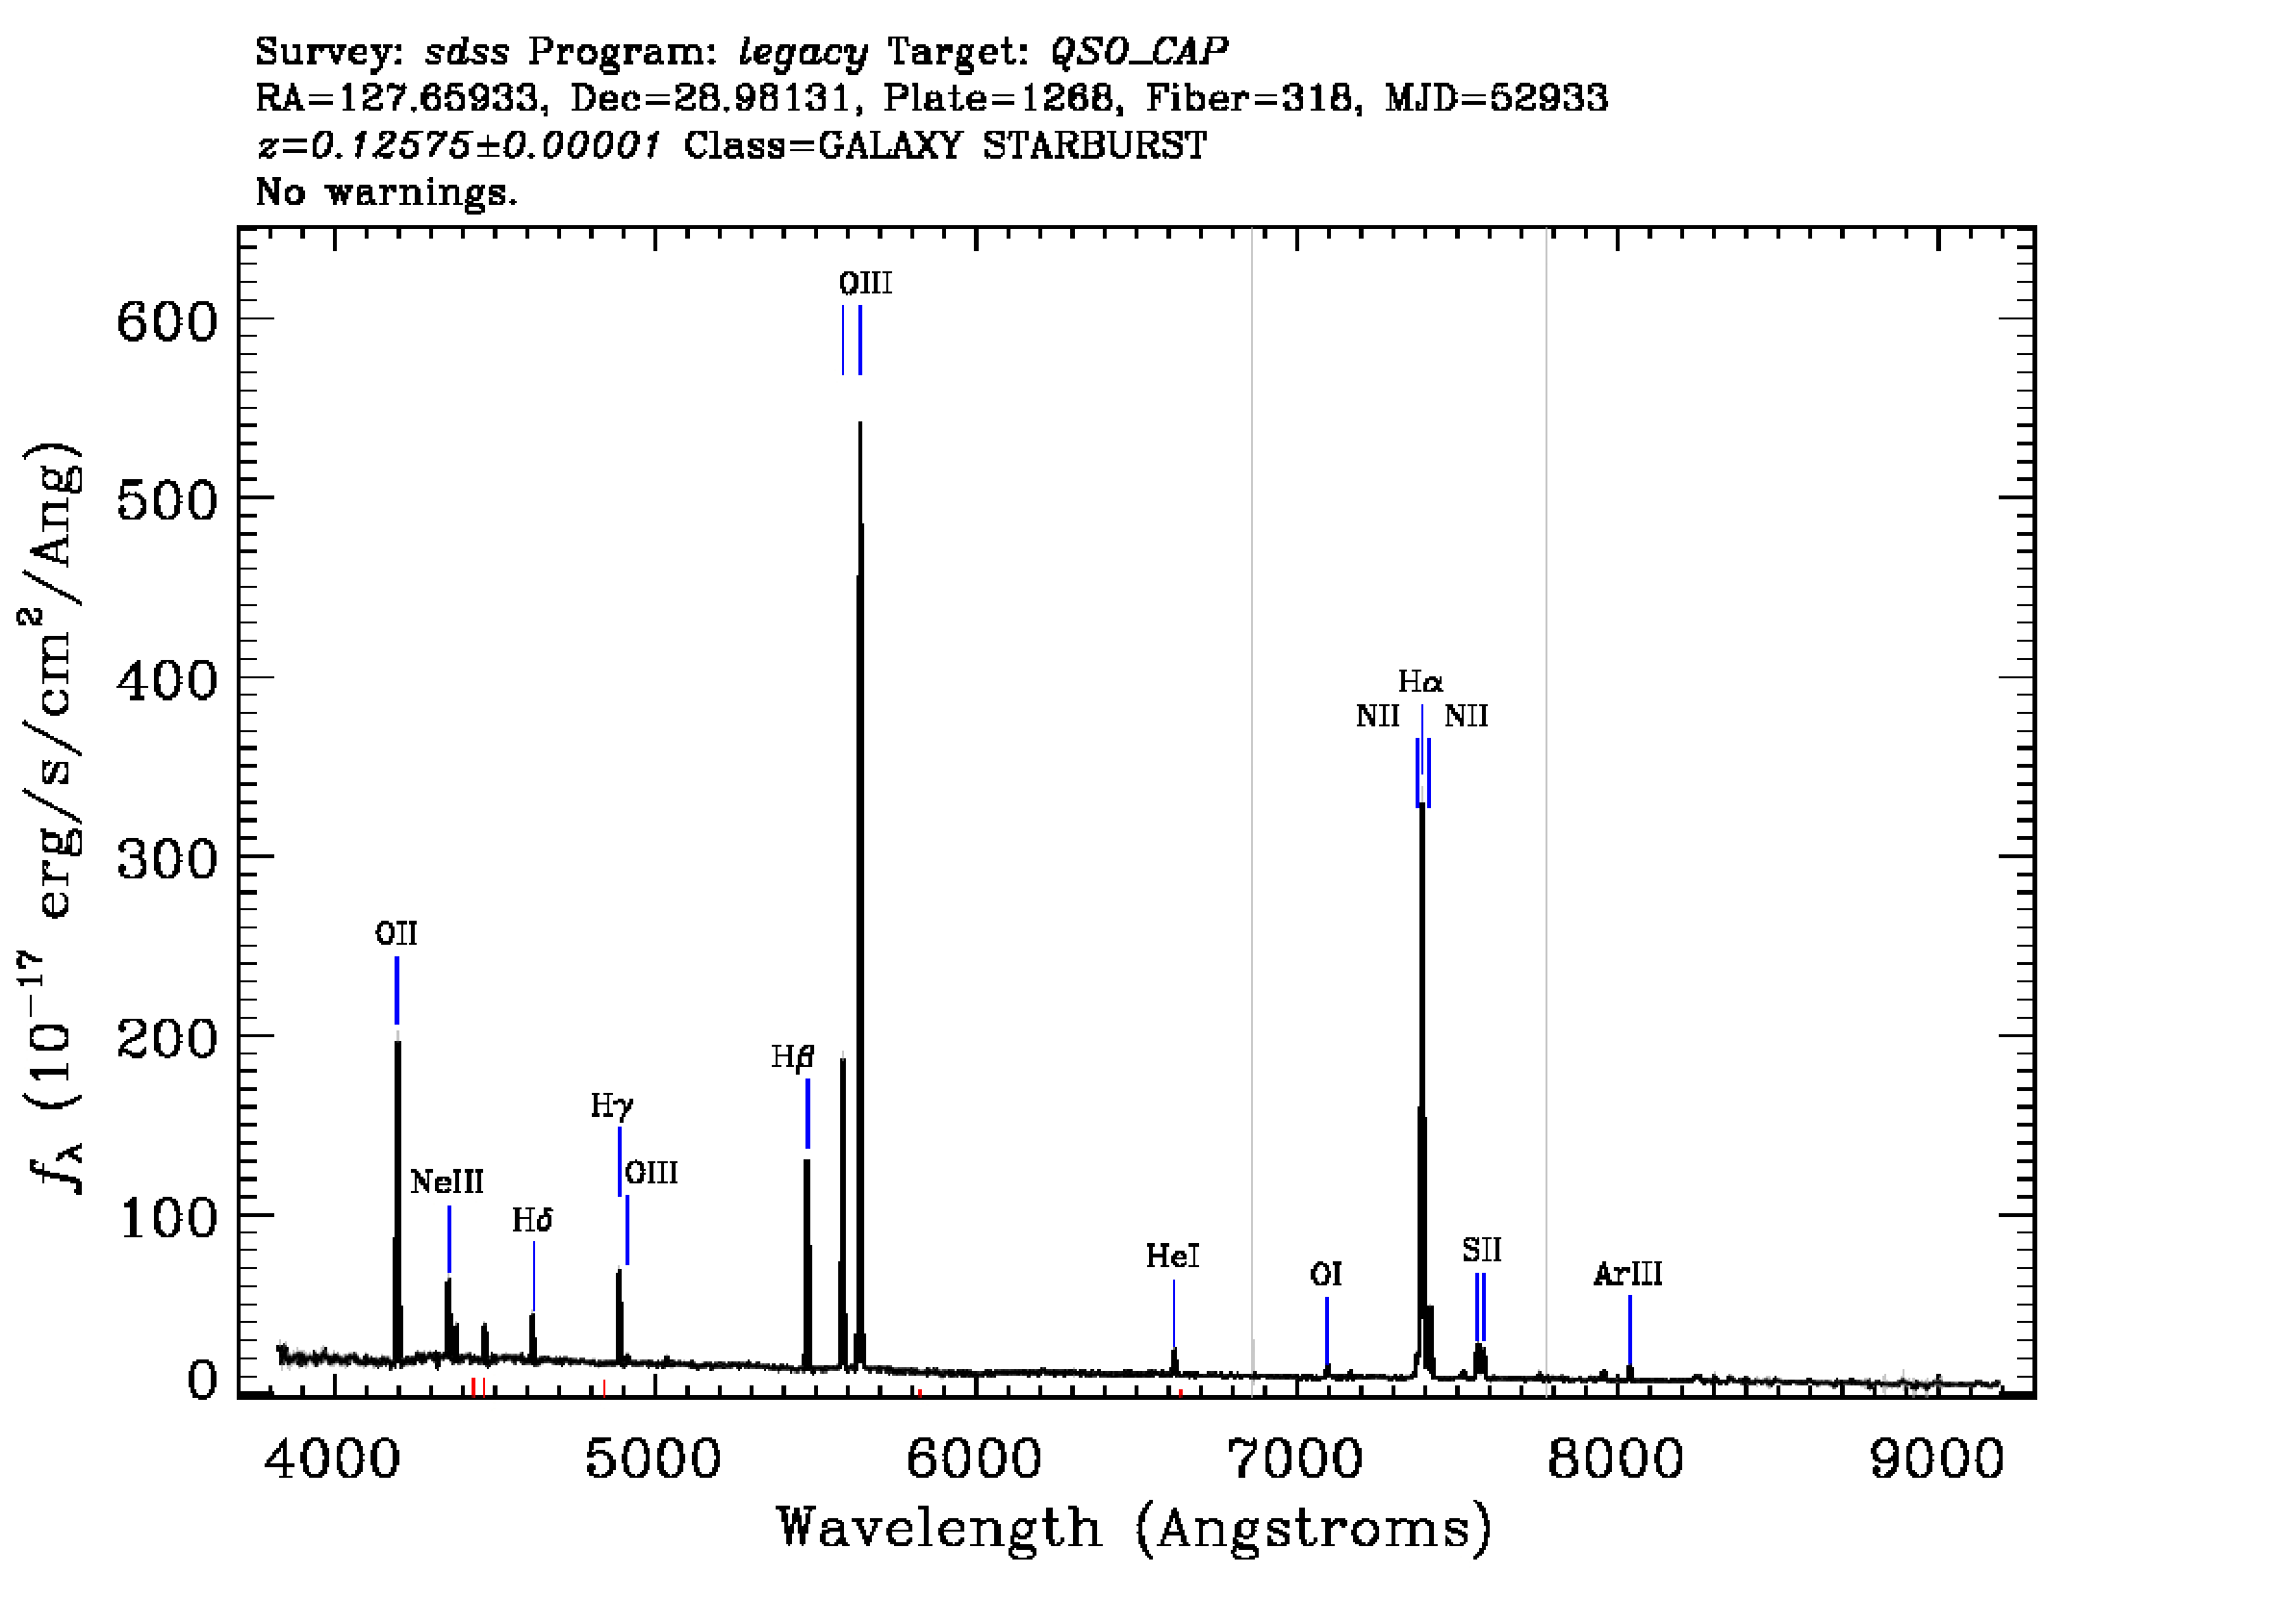
\includegraphics[scale=0.4]{SpecById.pdf} 
  % \plotone{SpecById.eps} 
   \caption{Spectrum of SDSS target specified by Plate~\#1268, Fiber~\#318 from the SDSS3 DR10.  \label{shsinput:fig}}
\end{figure}

We calculate the expected signal using the first order $m=1$ for a SHS with grating line density $1/d=1200$\,mm$^{-1}$.
Different configurations of the SHS are achieved by adjusting the grating tilt angle $\theta$, although swapping
gratings can achieve a similar effect.
The SHS configuration can then be expressed in terms of the Littrow wavenumber.  For the [OIII] doublet of
the target under consideration
the condition for having only one beat frequency occurs when $\sigma_0=\sigma_2=17913$\,cm$^{-1}$
occurs at $\theta=0.341551$.
Different choices of Littrow wavenumber
produce different output signals:
Figure~\ref{shscounts:fig} shows the expected counts adjusting $\sigma_0$ to produce beat frequency ratios
$n=1/3.5,1/1.05,1,1.05,3.5$ according to Eqn.\ \ref{littrowchoices:eqn}.
The maximum $x$ is chosen to be $(12s_1\tan{\theta})^{-1}$ in order to cover the decay caused by the line-width.
The effect on the signal
of the choice of the beat frequency of $2(\sigma_1+\sigma_2-2\sigma_0)\tan{\theta}$ relative to the $2(\sigma_1-\sigma_2)\tan{\theta}$ frequency
is clearly apparent.

\begin{figure}[t]
   \centering
   \plotone{shscounts.pdf} 
   \caption{The output signal for positive $x$ of the  SHS configurations that give the four different
   Littrow numbers according to
   $n=1/3.5,1/1.05,1,1.05,3.5$  in Equation~\ref{littrowchoices:eqn}. The output signal is symmetric about $x=0$.\label{shscounts:fig}}
\end{figure}

The redshift precision is estimated using a Fisher matrix with $z$ as the only free parameter. 
The baseline observation is for an 8-hour exposure on a 10-m telescope assuming a 70\% total
system transmission
with 2048 pixel samples. 
Blocking filters remove flux in wavelengths outside the regions
of interest.  The new moon CTIO sky emission is included but
is small compared to the galaxy continuum.
A circular aperture of $1\arcsec$ diameter is assumed to cover the full line flux.  Detector noise is taken to be negligible.
The precision is insensitive to the choice of $\sigma_0$, except
for small deviations near $n=1$ and at integer ratios of the beat frequencies; we choose
the case of $n=1.5$ or $\theta = 0.3421194$ (a change in angle of $1.95 \arcmin$ from the $n=1$ case)
as a representative example where the pixels resolve the frequencies of interest.
The redshift uncertainty from the [OIII] lines is then $\sigma_z^{[OIII]}=1.08\times 10^{-8}$
and correspondingly the [OII] lines give $\sigma_z^{[OII]}=2.39\times 10^{-8}$.  In a single observation
both doublets can be observed simultaneously with different interferometers combine to
give $\sigma_z^{[OII]\&[OIII]}=9.88\times 10^{-9}$.
This is over an order of magnitude improvement
of the high-precision redshift measurement of  $\sigma_z=6\times 10^{-7}$ obtained
from the radio absorption line in 3C~286 at $z=0.849$
\citep{1978ApJ...219....1D}.

The redshift uncertainty scales inversely with telescope aperture and the square root of exposure time;
a 40-m telescope provides a factor 4 and 800 hours integration a factor 10 improvement and a combination
of the two would give $\sigma_z=2.47\times 10^{-10}$. 

The SDSS3 DR10 database contains a number of emission line galaxies (ELGs) that could be targeted.
The redshift accuracy that can be achieved for galaxies in a range that extends  to $z=0.56$ with
an 8 hour exposure on a 10-m telescope
is given in Table~\ref{dz:tab}. 
Future spectroscopic surveys targeting ELGs, such as eBOSS and DESI, will provide a large catalog
from which to select galaxies with doublets that allow precision redshift measurement.
\begin{deluxetable}{cccccc}
\tablecaption{SHS Redshift Uncertainties of Select SDSS Targets With
an 8 Hour Exposure on a 10-m Telescope. \label{dz:tab}}
\tablehead{
\\colhead{Plate} &\colhead{Fiber} & $z$ &\colhead{$\sigma_z^{[OII]}$} & \colhead{$\sigma_z^{[OIII]}$} & \colhead{$\sigma_z^{[OII]\&[OIII]}$}
}
\startdata
1523 & 602 & 0.08933221 &\nodata & $2.4\times 10^{-8}$ &  $2.4\times 10^{-8}$ \\
1935 & 204 & 0.09838755 & $1.7\times 10^{-8}$ & $7.9\times 10^{-9}$ & $7.2\times 10^{-9}$  \\
1036 & 584 & 0.1078989 &  \nodata & $4.2\times 10^{-8}$ &  $4.2\times 10^{-8}$ \\
2959 & 354 & 0.1199353 &  \nodata & $9.5\times 10^{-8}$ &  $9.5\times 10^{-8}$ \\
1268 & 318 & 0.1257486 & $2.5\times 10^{-8}$ & $1.1\times 10^{-8}$ & $1.0\times 10^{-8}$  \\
1657 & 483 & 0.2213398 & $3.1\times 10^{-8}$ & $1.6\times 10^{-8}$ & $1.4\times 10^{-8}$  \\
1073 & 225 & 0.2716023 & $8.7\times 10^{-7}$ & $1.3\times 10^{-8}$ & $1.3\times 10^{-8}$  \\
1514 & 137 & 0.318046 & $5.5\times 10^{-8}$ & $1.3\times 10^{-7}$ & $5.0\times 10^{-8}$  \\
4794 & 757 & 0.5601137 & $6.6\times 10^{-7}$ & $9.0\times 10^{-7}$ & $5.3\times 10^{-7}$  \\
1059 & 564 & 0.693329 &  $1.6\times 10^{-8}$ &  \nodata &  $1.6\times 10^{-8}$
\enddata
\end{deluxetable}

The long exposures could be divided into sub-exposures each with a different SHS configuration, either my changing the
gratings or by rotating the grating angles with a series of $\delta \theta$.
Using many configurations desensitizes the result from potential systematic uncertainties:
the high-frequency wiggles characteristic to each configuration
are insensitive to the imperfectly-known line profiles that define the common envelope;
the redshift measurement is dependent on many pixels and any single pixel contributes a different weighting to the redshift measurement,
as a result the measurement  is less sensitive to
detector miscalibration; with precisely known changes to $\theta$ or $1/d$, the absolute $\theta$ calibration can
be fit out. 

In the regime under consideration, the redshift precision goes inversely with the line width and the inverse square of line flux.

\section{Externally Dispersed Interferometer}
The Externally Dispersed Interferometer \citep[EDI;][]{2003PASP..115..255E} is a candidate instrument with which to measure precision redshifts.
An EDI is the sequence of a Fourier transform spectrograph (FTS) and a dispersion spectrograph.  The FTS is an interferometer that shifts
the phase of incoming coherent light, 
by an amount dependent on wavelength and the relative arm lengths.
The ensuing dispersion spectrograph takes the incoming light and separates them into fine wavelength bins.
For an individual wavelength bin the output signal depends on the phase introduced by the interferometer; multiple
measurements taken after adjusting the arm-lengths make apparent a modulation in the output signals.
Therefore, in an EDI the wavelength can be measured using the calibration methods of a standard dispersion
spectrograph {\it and} from the modulations of signal apparent when changing the FTS arm-lengths.

An EDI produces measurements that can be related
to a conventional spectrum
\begin{equation}
B(\nu) = S_0(\nu) \otimes \mbox{PSF}(\nu),
\end{equation}
and an independently measureable whirl
\begin{equation}
W(\nu) = \frac{1}{2}\left[e^{i2\pi\tau_d\nu}S_0(\nu)\right] \otimes \mbox{PSF}(\nu),
\end{equation}
where $S_0$ is the input spectrum, $\tau_d$ is the interferometer delay, and $\mbox{PSF}$  is the blurring
response of a pure frequency.

The heterodyning feature of the EDI is seen in the Fourier transforms of the above expressions:
\begin{align}
b(\rho) & =s_0(\rho) \, \mbox{psf}(\rho)\\
w(\rho -\tau_d) & =\frac{1}{2} s_0(\rho) \, \mbox{psf}(\rho-\tau_d).
\end{align}
The EDI whirl has the instrumental frequency response shifted into a new $\rho$ range to allow
spectral
resolution on scales tuned by the choice of $\tau_d$.

An EDI observation of image $i$ is actually a series of measurements
\begin{equation}
B(\nu)_{i,\Delta\phi} = \left[\left[S_i(\nu)\left(1+\cos{\left(2\pi\tau\nu+\phi_y+\Delta\phi \right)} \right)\right]\otimes \mbox{PSF}(\nu)\right]\Sha\left(\frac{\nu}{p}\right),
\end{equation}
where $p$ is the spacing of the frequency sampling, $\phi_y$ is the initial phase, $\Sha$ specifies the discrete sampling,
and the phase shifts $\Delta\phi$ could be chosen as
$0$, $\pi/2$, $\pi$, and $3/2\pi$ for later calculational simplicity.

The redshift precisions on the galaxies considered in \S\ref{SHS:sec} are given in Table~\ref{dz_edi:tab}
for four 2-hour exposures on a 10-m Telescope with 70\% throughput.  For the FTS we
chose a value of $\tau=(3\Delta \sigma)^{-1}$, where 
\begin{equation}
\Delta \sigma = \frac{(\sigma_{10}+\sigma_{20})}{2}\left((1+z)^{-1}-(1+z+10^{-9})^{-1}\right)
\end{equation}
is the expected change in the average wavenumber of the two lines given a shift in redshift of $10^{-9}$,
and the factor 3 is found to give good sensitivity.
The dispersion spectrograph has a per-pixel $R=20000$.  The line-spread-function $\mbox{PSF}$ is a top-hat function defined by a wavelength
resolution bin.  Each doublet is considered on its own, {\it Total} precision has contribution from the {\it Conventional} spectrum and the {\it Whirl}; each is
is tabulated.  The last column shows the combined constraint from both doublets assuming multiplexing, either through one or two EDI's.
Almost all the constraining power comes from the whirl and the total precisions are several factors better than with the SHS.

\begin{deluxetable}{cccccccccc}
\tabletypesize{\scriptsize}
\tablecaption{EDI Redshift Uncertainties of Select SDSS Targets With
an 8 Hour Exposure on a 10-m Telescope. \label{dz_edi:tab}}
\tablehead{
\colhead{} &\colhead{} &\multicolumn{3}{c}{[OII]}&\colhead{} &\multicolumn{3}{c}{[O|II]}&\colhead{[OII] \& [OIII]} \\
\cline{3-5} \cline{7-9}\\
\colhead{Plate} &\colhead{Fiber} & \colhead{Total} & \colhead{Conventional} & \colhead{Whirl} &\colhead{} &  \colhead{Total} & \colhead{Conventional} & \colhead{Whirl}  & \colhead{Total}
}
\startdata
1523 &602 &\nodata&\nodata &\nodata && $6.6\times 10^{-9}$ & $6.8\times 10^{-8}$ & $6.6\times 10^{-9}$ & $6.6\times 10^{-9}$\\
1935 &204 &$5.2\times 10^{-9}$ & $4.8\times 10^{-8}$ & $5.3\times 10^{-9}$ && $2.1\times 10^{-9}$ & $1.9\times 10^{-8}$ & $2.1\times 10^{-9}$ & $1.9\times 10^{-9}$\\
1036 &584 &\nodata&\nodata &\nodata& & $8.7\times 10^{-9}$ & $1.0\times 10^{-7}$ & $8.8\times 10^{-9}$ & $8.7\times 10^{-9}$\\
2959 &354 &\nodata&\nodata &\nodata& & $2.1\times 10^{-8}$ & $1.9\times 10^{-7}$ & $2.1\times 10^{-8}$ & $2.1\times 10^{-8}$\\
1268 &318 &$7.3\times 10^{-9}$ & $6.7\times 10^{-8}$ & $7.4\times 10^{-9}$ & &$2.8\times 10^{-9}$ & $2.6\times 10^{-8}$ & $2.8\times 10^{-9}$ & $2.6\times 10^{-9}$\\
1657 &483 &$8.8\times 10^{-9}$ & $8.1\times 10^{-8}$ & $8.8\times 10^{-9}$ & &$3.8\times 10^{-9}$ & $3.5\times 10^{-8}$ & $3.9\times 10^{-9}$ & $3.5\times 10^{-9}$\\
1073 &225 &$2.3\times 10^{-7}$ & $2.3\times 10^{-6}$ & $2.4\times 10^{-7}$ & &$2.8\times 10^{-9}$ & $1.0\times 10^{-7}$ & $2.8\times 10^{-9}$ & $2.8\times 10^{-9}$\\
1514 &137 &$1.5\times 10^{-8}$ & $1.4\times 10^{-7}$ & $1.5\times 10^{-8}$ & &$1.7\times 10^{-8}$ & $1.5\times 10^{-7}$ & $1.7\times 10^{-8}$ & $1.1\times 10^{-8}$\\
4794 &757 &$1.8\times 10^{-7}$ & $1.8\times 10^{-6}$ & $1.8\times 10^{-7}$ & &$9.7\times 10^{-8}$ & $9.6\times 10^{-7}$ & $9.7\times 10^{-8}$ & $8.5\times 10^{-8}$\\
1059 &564 &$5.4\times 10^{-9}$ & $4.9\times 10^{-8}$ & $5.4\times 10^{-9}$ & &\nodata  & \nodata & \nodata & $5.4\times 10^{-9}$\\
\enddata
\end{deluxetable}


Euclid where to find sources.

\bibliographystyle{apj}
\bibliography{/Users/akim/Documents/alex.bib}

\end{document}